\chapter{Analysis of collected data}\label{analysis_collected_data}
    In order to perform some experiments using the learning framework proposed and described in \ref{learning_framework}, one needs to obtain training data. These data should be
    \begin{itemize}
        \item Abundant. The more data, the better.
        \item Consistent. Ideally, data are not mutually opposed --- i.e., they are not contradictory.
        \item Reliable. Data should come from reliable sources, since erroneous or inaccurate information affect the performance of machine learning algorithms.
    \end{itemize}
    In general, data quality should be high.
    
    In this chapter, I describe how data have been collected through the labelling platform, and I analyze what has been collected from quantitative and qualitative perspectives.
    \section{Data collection}
        Data collection --- i.e., the process of gathering and measuring data --- is a very important step in a data science project, especially when dealing with a (semi-)supervised machine learning algorithm.
        
        In this thesis setting, data comes in the form of labelled Wikipedia pages. In other words, the learning framework I have proposed and tested needs to know what are the labels of some Wikipedia pages. This data is then used to propagate information to all the other vertices of the Wikipedia graph. Specifically, according to the strategy followed in this thesis (described in section \ref{solution_overview} and \ref{experiments_chapter}), only Wikipedia category pages have been classified: there are no enough computational resources to run the learning framework on the entire Wikipedia articles graph, and there are only few participants that have volunteered with the labelling task (see section \ref{participants}).
        
        The tool I have used to collect data is the web interface of the labelling platform presented and described in chapter \ref{labelling_platform}. Since it has been built keeping usability in mind, such interface can be used by anyone.
        \subsection{Label set}
            Before starting with data collection, one must fix an arbitrary set of labels to choose from. Indeed, the learning framework needs to know in advance which are the categories every node of the Wikipedia graph can be assigned to.
            
            I have decided to experiment with the same categories used in Negapedia. In this way, it is somehow possible to compare the results of the learning framework with those obtained with the algorithm developed by \citeauthor{Bonetti} in \cite{Bonetti}. Here is category list:
            \begin{multicols}{2}
                \begin{itemize}
                    \item Culture, arts and entertainment
                    \item Geography and places
                    \item Health and fitness
                    \item History and events
                    \item Mathematics and logic
                    \item Nature and physical sciences
                    \item People and self
                    \item Philosophy and thinking
                    \item Religion and belief systems
                    \item Society and social sciences
                    \item Technology and applied sciences
                \end{itemize}
            \end{multicols}
        \subsection{Participants}\label{participants}
            The second step of the data collection process is recruiting participants willing to volunteer. However, as is often the case, it was not easy to find out an appropriate number of participants.
            
            A total of thirteen participants have helped with the labelling task. They come from five different countries (Italy, Germany, Netherlands, Poland and United States) and labeled pages only in their native language. An exception was made for the English Wikipedia --- which has been labeled also by non-native English speakers --- since it is considered to be an international version accessed from all over the world. I want to point out that all participants come from countries where Wikipedia is well developed and have more than one million articles\footnote{\url{http://meta.wikimedia.org/wiki/List_of_Wikipedias}.} (in fact, they are in the top ten list by article count\footnote{\url{http://meta.wikimedia.org/wiki/Top_Ten_Wikipedias}.}).
            
            \begin{table}[h]
                \centering
                \begin{tabular}{|c|c|}
                    \hline
                    Spoken language & Number of participants \\ \hline \hline
                    English & 11 \\ \hline
                    Italian & 5 \\ \hline
                    German & 3 \\ \hline
                    Polish & 3 \\ \hline
                    Dutch & 1 \\ \hline
                \end{tabular}
            \end{table}
            
            With regard to the queries posed by the active learner, it was basically impossible to find volunteers, since they have helped only during their spare time. Therefore, I had to personally answer the queries of the active learner, thus limiting its capacity to my budget (in terms of time) and to the languages I am comfortable with (English and Italian). 
        \subsection{Data summary}
            Here is a summary of data collected through the web interface of the labelling platform. Data collected during the active learning process has been neither quantified nor stored anywhere. In fact, there have been many trials to test the functionality of the learning framework, and I have labeled many pages during each of them. However, keep adding labels to the initial training set would have improved the performance of the learned model and would have given it an advantage over previous models. Therefore, I decided to keep the initial training set fixed and I have used only the labels collected through the help of other participants.
            
            \begin{figure}
                \centering
                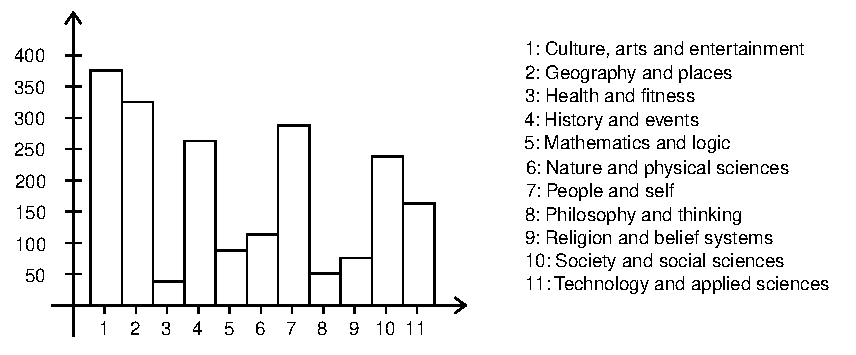
\includegraphics[width=0.9\textwidth]{images/data_histogram.pdf}
                \caption{Bar chart representing how many times each label has been used by participants to classify one of the category pages of Wikipedia. Data are related to several different Wikipedia versions --- i.e., English, Italian, German, Polish and Dutch. Moreover, some pages may have been labeled multiple times by different persons.}
                \label{data_histogram}
            \end{figure}
            % 375, 325, 40, 255, 90, 105, 280, 50, 70, 240, 150 = 1980
            
            Data collected by the participants are summarized in figure \ref{data_histogram}. As you can see, almost 400 category pages have been labeled as \textquote{culture, art and entertainment}, while less than 50 have been labeled as \textquote{health and fitness} (almost 2000 collected labels). This is probably due to the fact that most of the pages are likely to be grouped under some wide categories. However, some participants have pointed out another problem: there are cases in which they are unable to classify some pages because they cannot understand what these categories are about.
            
            I also have to point out that some pages have been labeled multiple times. I decided to make such a choice because I wanted to check whether different people classify the same page in different ways --- i.e., they classify the same page with different labels. Therefore, the amount of collected labels does not correspond to the total number of labeled category pages.
            
            With regard to the number of collected labels per language, English was of course the Wikipedia version where I was able to collect more data, since most of the participants are familiar with that language. It was also interesting to collect data regarding Polish and Dutch Wikipedia, since to the best of my knowledge no one has ever tried to include such versions in a multilingual classifier of Wikipedia pages. Results are summarized table \ref{labels_by_language}.
            
            \begin{table}[h]
                \centering
                \begin{tabular}{|c|c|}
                    \hline
                    Spoken language & Number of collected labels \\ \hline \hline
                    English & 612 \\ \hline
                    Italian & 490 \\ \hline
                    German & 378 \\ \hline
                    Polish & 324 \\ \hline
                    Dutch & 176 \\ \hline
                \end{tabular}
                \caption{Number of collected labels on different Wikipedia versions.}
                \label{labels_by_language}
            \end{table}
            % 1980 in totale
    \section{Data comparison}
        Some of the pages that have been labeled 
        In this section, I compare data related to different languages to understand if participants coming from different countries label the same semantic concept in different ways. Moreover, this section tries to understand what are the differences between the Negapedia algorithm and the manually collected data.
        \subsection{Differences between different Wikipedia versions}\label{difference_between_wikipedias}
            Some pages written in different languages are connected through a langlink (see section \ref{langlinks} for more details). In particular, some of these pages form a complete graph\footnote{A graph in which two vertices are connected by a bi-directional langlink, for every pair of distinct vertices.}. Therefore, they are likely to be related to the same semantic concept, and they can be thought of as the same page.
            
            Are these pages labeled in the same way? Do participants coming from different countries label a page in the same way? Answers to these questions may help to solve a more general problem: are langlinks reliable when used to model semantic identity? The quality of the learning framework presented in this thesis strongly depends on this answer.
            
            \begin{figure}
                \centering
                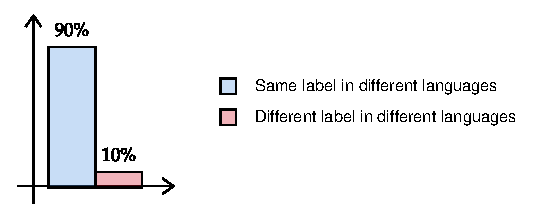
\includegraphics[width=0.8\textwidth]{images/comparison_wikipedias.pdf}
                \caption{The chart displays the percentage of pages that have been labeled consistently by participants speaking different languages. Only pages that come from five different languages (English, Italian, German, Polish and Dutch) and that form a complete graph with their langlinks are taken into account. Moreover, cases in which participants that speak the same language disagree are discarded.}
                \label{comparison_wikipedias}
            \end{figure}
            
            It turned out that most of the times the category assigned to a Wikipedia page does not depend on the language of the volunteer who performed the labelling task (in fact, those differences are referable to intrinsic data uncertainty, described in section \ref{sec_uncertainty}). As one can easily see from image \ref{comparison_wikipedias}, if participants that speak the same language agree on the label to assign to a page then the same thing holds for different volunteers that speak another language. This specific situation occurred only twenty times: I cannot trust these percentages too much. However, when I tried to further analyze the two cases in which different labels were assigned to these pages, I found out that in both cases there was a mistake in a single language made by a participant. Therefore, using the few data I had, I can conclude that a complete graph created with langlinks is likely to represent the same concept.
            
            If one takes pages that are not fully connected then the results get a bit worse: a higher percentage of pages belonging to different Wikipedia versions are classified in different ways. In particular, I have found out that 30\% of such pages have this problem. This is probably due to the fact that sometimes the same concept is described using a single page in a Wikipedia, and multiple pages in another one. Probably, one could show that there is a relationship between the connectivity strength of the langlinks graph and the consistency of classification, but I do not have enough data to prove it.
        \subsection{Differences between collected data and Negapedia}
            Only relatively few labels have been gathered, but the learning framework needs many more if one wants to achieve a good performance. Therefore, a new data source must be found in order to get other training labels. Negapedia and the algorithm developed in \cite{Bonetti} may be an option: it would be interesting to know whether there are similarities between data collected using the labelling platform and those provided by Negapedia. Is data coming from Negapedia reliable?
            
            The algorithm developed by \citeauthor{Bonetti} can in principle work for any language. However, it has two major drawbacks:
            \begin{itemize}
                \item It has to be separately tuned for each language. Hence, it needs experts that validate its results. Currently, it directly support only English and Italian, while partial support to other languages is obtained by propagating information through langlinks.
                \item Since Italian and English Wikipedia versions have been independently tuned, sometimes they may provide different results, even when two pages are fully connected with langlinks and represent the same semantic concept.
            \end{itemize}
            
            Since Negapedia is optimized only for English and Italian, I decided to take into account only data coming from those two languages, ignoring the others.
            
            The algorithm makes some bad mistakes compared to human evaluation --- such as classifying the English categories \textquote{Trojan War} and \textquote{Greek mythology} respectively as \textquote{mathematics and logic} and \textquote{geography and places}.
            
            In general, the algorithm and the collected data disagree almost 35\% of times. However, we must distinguish between two kinds of mistakes:
            \begin{itemize}
                \item If participants disagree --- i.e., they classify the page in different ways --- and the algorithm makes a mistake, then this mistake is somehow less bad, since humans themselves are not able to agree and the example is probably difficult to classify.
                \item On the other hand, if participants agree --- i.e., they classify the page in the same way --- and the algorithm makes a mistake, then this mistake is somehow worse, because volunteers agree and therefore the example is likely to be easier to classify. In this kind of mistake, all the cases in which only one label was collected are not included (there must be at least two answers for the same page).
            \end{itemize}
            These results are reported and summarized in table \ref{negapedia_errors}.
            
            \begin{table}[]
                \centering
                \begin{tabular}{cc|c|c|}
                    \cline{3-4}
                    & & \multicolumn{2}{c|}{\textbf{Algorithm}} \\ \cline{3-4} 
                    & & Correct & Wrong \\ \hline
                    \multicolumn{1}{|c|}{\multirow{2}{*}{\textbf{Users}}} & Agree & 35 & 6 \\ \cline{2-4} 
                    \multicolumn{1}{|c|}{} & Disagree & 120 & 44 \\ \hline
                \end{tabular}
                \caption{Given Italian and English category pages for which there are at least two labels, when does the Negapedia algorithm make a mistake? The table displays a relationship between user agreement and the algorithm performance.}
                \label{negapedia_errors}
            \end{table}
            % 612 inglese, 490 italiano = 1102 totale
            % 107 ripetute in inglese, 98 in italiano = 205 totale
            % 50 sbagliate in totale, rimanenti 155 giuste
            
            Though sometimes the algorithm is wrong, most of the mistakes come from situations in which participants answered in different ways, without finding an agreement. This is somehow acceptable, because an algorithm is unlikely to perform better than a human in this task.
            
            Moreover, if one analyze the many mistakes made by the algorithm when users disagree, it is possible to notice that most of them are not very bad: many times the algorithm classify a category which lists people with the label closer to what such people do (for example, instead of labelling the page \textquote{Category:Chess players} as \textquote{people and self} --- as the participants did --- the algorithm classifies it as \textquote{culture, arts and entertainment}, which is not completely wrong).
            
            Finally, I noticed that most of the errors made by the algorithm come from situations in which the algorithm itself was unsure about the result. Indeed, Negapedia computes a probability distribution over the topics, and keep the one with highest score. If the score is not very high, then the answer given by the algorithm has higher chances to wrong.
            
            I can conclude that it is perfectly fine to use such data while training a model with the learning framework:
            \begin{itemize}
                \item Though there are some normal mistakes made by the algorithm behind Wikipedia, they mostly come from situations in which users tend to disagree.
                \item Misalignment between collected data and answers given by the algorithm are likely to happen when the algorithm returns a low highest score in the probability distribution.
            \end{itemize}
            %1487200 -- Category:Trojan War -- Mathematics
            %691702 -- Category:Greek mythology -- Geography
            %691724 -- Category:Chess players -- Culture
    \section{Data reliability}
        While figure \ref{data_histogram} may have represented the real distribution over topics, the values in the bar chart are probably greatly influenced by the background of the chosen participants.
        
        Sometimes they are simply unable to classify some pages because they do not know what they are about and, in general, they are not comfortable with the topic:
        \begin{itemize}
            \item If they try to answer with a label even if they are unsure, they could make a mistake, thus introducing errors in the training set. The learning framework is likely to propagate these errors to other pages and/or to other languages.
            \item On the other hand, if they decide not to answer, the distribution of the training set could change substantially, because they would only give answers related to their field of expertise, thus introducing some bias in the data.
        \end{itemize}
        
        In my experiments, I asked the participants not to answer if they were not sure about the label to assign. Indeed, I think that having errors --- and, above all, propagating them --- is worse than having a distribution which does not reflect the reality. This is largely motivated by the fact that errors are difficult to be found once they are in the training set (especially if I am not comfortable with the language), while unlabeled pages can be kept aside and assigned to someone else.
    \section{Data uncertainty}\label{sec_uncertainty}
        Pages connected by a langlink may be labeled in different ways. The reason behind this situation could be a wrong link --- i.e., a langlink that connects two pages related to different concepts, as pointed out in section \ref{difference_between_wikipedias}. However, what about pages that are assigned to different topics by participants that speak the same language? What are the reasons and what can we do about such situations?
        
        While differences between languages can be caused by wrong langlinks (mistakes made by Wikipedia contributors), the cause of multiple different classifications of a page in a given language must be searched somewhere else. In particular, there might be concepts which cannot be clearly classified as belonging to a certain category or another: it is very difficult --- and probably impossible --- to create non-overlapping categories which comprise all the existing concepts.
        
        Also, the ultimate practical goal of having a tool which is able to classify Wikipedia pages is to provide users of a website like Negapedia with a method to navigate articles. If users are unsure about the correct classification of a given article, there is no way one can create a universal taxonomy accessible by anyone: there will always be people who think an article should be under a different category. The only thing one can do is to trust the wisdom of the crowd, and try to select the category which has a majority\footnote{One could also try to personalize results, but that is a completely different problem (and much more difficult).}.
        
        Some examples of pages in a given language which are classified in different ways by participants can be found in table \ref{uncertainty}.
        
        \begin{table}
            \centering
            \begin{tabular}{|l|l|l|}
                \hline
                Pages                     & Label A                         & Label B              \\ \hline \hline
                Israelites                & History & People \\ \hline
                Fictional characters      & Culture & People      \\ \hline
                East Germany              & History            & Geography \\ \hline
                Catholic pilgrimage sites & Religion    & Geography \\ \hline
            \end{tabular}
            \caption{Some examples of Wikipedia pages which have been classified in different ways by participants that speak the same language. It is not easy to what the \textquote{right} label should be, since the ultimate goal is to create a useful tool for users.}
            \label{uncertainty}
        \end{table}
        
        To conclude, whenever a page is classified in different ways, and once one is sure that such misalignment is not caused by human errors but only by different interpretations, it is possible to keep these differences and take into account what the majority thinks.